\chapter{Method 1: sequential information extraction}%Panel extraction}
\chaptermark{Sequential information extraction}
\label{chap:sequential}
\graphicspath{{./chapters/3-sequential/figs/}}

% Abstract -------------------------------------------------------------------------------------------------------------------------------------------
This chapter presents a sequential information extraction approach for comic book content retrieval.
The sequence of extraction starts from elementary elements such as panel and text that initiate further processing.
Once the text regions are discovered, we use them as seeds to search for balloons and then analysis the balloon contours to detect the tails.
From the tail, comic character regions are computed according to previously extracted element positions.

% -------------------------------------------------------------

\section{Introduction} % (fold)
\label{sec:introduction}

In comics art, the page structure depends on the author style, this is why so many different structures and drawing types exist.
It is unavoidable because it gives an unique graphical identity to the comics and contributes to attract the curiosity of the readers.
Despite the differences of style, the comics drawings follow ``general use'' characteristic intrinsically to the design process~\cite{mccloud2006Making}.
% Relations between elements and inking process are particularities that we we rely on when processing such images. surrounded by a black stroke.
For instance, the inking process requires to magnify the main strokes and then colourize.
We propose to rely on this main strokes to automatically extract non coloured image content (e.g. panel boundary, text, speech balloon background) using a connected-component labelling~\cite{Szeliski2010Computer} approach.
Then, the analysis of speech balloon contour allows to detect the tail precisely and its direction is used to compute the regions of interest where comic characters are supposed to be.
In this section, all the processes are related to each other, for instance, the text extraction output is the input of the balloon extraction process.


% section introduction (end)

\section{Panel and text} % (fold)
\label{sec:se:panel_and_text}


This section proposes a method to automatically extract the panels and text regions contained in comics pages.
This method is not limited to text which is included into speech balloon such as most of the work in the literature.
Here we consider all the text regions of the image using connected-component labelling approach and k-means clustering.

% \p{Methodology} % (fold)
% \label{sec:se:methodology}

To be clustered, the connected components have to be extracted from the image first.
A commonly used method is to segment the original image pixels into two categories called foreground and background.
The foreground category corresponds to the set of pixels of interest, here the pixels of the panel border strokes.
The background includes other pixels.
This is usually performed using binary segmentation techniques which assign each pixel to one of the two categories.
From the foreground pixels, a structural analysis (connected-component labelling) allows us to group ``connected'' pixels into components according to their connectivity.
 % that are connected (black pixels over white background).
% Then, the ROI are defined as the set of the connected-component bounding boxes (rectangles).

% Connected components labelling scans an image and groups its pixels into components based on pixel connectivity.
% All pixels in a connected component share similar pixel intensity values and are in some way connected with each other.
Connected component approaches are commonly used for stroke-based document analysis, there are also simple and computationally efficient.
Once extracted, their can be clustered according to different features (e.g. size, shape ,colour, location).
We use this approach to extract panels and text which can be easily differentiated using size and topological information.
% with meaningful names ``noise'', ``text'' and ``panel'' using a classifier with three cluster using discriminant features for instance.
% The originalities of this paper are frame segmentation, with or without box, and out-of-balloon text segmentation that can be extracted by CC algorithm.
% The aim of the pre-processing step is to separate background and content of the page in order to focus on the content later. Several processing are implemented in order to apply CC algorithm, and then, to extract the bounding boxes. It can be resumed as follows:
The process can be summarize as bellow:
  \begin{enumerate}
	\item Image segmentation
	\item Connected-component extraction
	\item Connected-component clustering
	\item Candidate regions pruning
  \end{enumerate}
% paragraph principle (end)


\paragraph{Image segmentation} % (fold)
\label{par:se:image_segmentation}

The first step consists in a colour to grey level (3 to 1 channel) conversion.
Several methods exits for such conversion, combining the three channels of the red, green, blue (RGB) colour space with different preponderation as given in~\cite{Pratt91} or using one channel from the Hue Saturation Lightness (HSL) or Value (HSL) representation of the RGB colour space.
Here we use the lightness channel because the panel border strokes and text are usually darker than other element in the image, including the background. 
Then, a global binary segmentation~\ref{??} (figure~\ref{fig:se:binary_img}) is applied with a threshold determined dynamically.
The threshold is computed from the median value of the border page pixels where pixels with a value lower than the median value are considered as part of the foreground (we are interested in black strokes).
We assume that the border pixels of the page are representative of the page background (depending on the digitization process).
If the median value is closer to ``black'' than ``white'' grey level, then, image inversion is applied and we redo the complete process in order to always get a white background at the end of this step.
% This pre-processing is more robust than~\cite{Arai11} who assumes that the page is always white and uses a constant threshold.
The binary conversion step is very important for the rest of the method because the background part will not be considered for further processing. %Sometimes, parts of text can be merged with background if their background intensity level is higher than the binarisation threshold.


\paragraph{Connected-component extraction} % (fold)
 \label{par:connected_component_extraction}
 
The connected-component algorithm~\ref{??} is applied on the binary image and the bounding box of each black component is computed to facilitate subsequent processing (Figure \ref{fig:se:cc_bounding_box}).
We do not consider white connected-component here because we assume that panel border and text elements are darker than other elements in the page (segmented as black region).

	%%%%%%%%%%%%%%%%%%%%%%%%%%%%%%%%%%%%%%%%%%%%%%%%%%%
	\begin{figure}	%trim=l b r t  width=0.5\textwidth, 
	  \centering
		%\includegraphics[height=60mm]{figure/BUBBLEGOM_T01_P007_crop.jpg}
		%\includegraphics[trim= 0mm 0mm 0mm 0mm]{figure/BUBBLEGOM_T01_P007.jpg}
		\subfloat[Binary segmented image]{\label{fig:se:binary_img}\includegraphics[trim= 0mm 0mm 0mm 0mm, clip, width=0.4\textwidth]{binary.png}}	\hspace{2em}
		\subfloat[Connected-component bounding boxes]{\label{fig:se:cc_bounding_box}\includegraphics[trim= 0mm 0mm 0mm 0mm, clip, width=0.4\textwidth]{roi.png}}
		\\
		\subfloat[Panel cluster]{\label{fig:se:frame_unrecognized}\includegraphics[trim= 1mm 0mm 0mm 0mm, clip, width=0.4\textwidth]{frame_unrecognized.png}}	\hspace{2em}
		\subfloat[Text cluster]{\label{fig:se:frame_cleaned}\includegraphics[trim= 1mm 0mm 0mm 0mm, clip, width=0.4\textwidth]{text.png}}
		  \caption[Panel extraction process]{Panel extraction process. Image credits:~\cite{Bubble09}.}
		  % \label{fig:se:binary_to_bounding_box}
	\end{figure}
	%%%%%%%%%%%%%%%%%%%%%%%%%%%%%%%%%%%%%%%%%%%%%%%%%%%

% paragraph process (end)

 % paragraph connected_component_extraction (end) 


\paragraph{Clustering} % (fold)
\label{par:clustering}
By looking at the figure~\ref{fig:se:cc_bounding_box}, we can clearly see that the bounding boxes of the panel are bigger than the others.
Also, they include more regions than others.
Classifying those regions according to their size allows us to classify panel and text region at the same time while ignoring noise information.
Knowing the number of cluster facilitate the clustering, here 
% The classification of connected-component heights using k-means algorithm. 
%We define the set of component bounding boxes $R = \{R_1, R_2, ... , R_n\}$.
we set the number of clusters $k=3$ according to the domain knowledge of comics.
They aim to reflect the ``panel'' (the highest), the ``text'' (medium height) and the ``noise'' (few pixels height) as shown on figure~\ref{fig:se:histo_roi}.
One of the most popular clustering algorithm is k-means clustering method~\ref{??}.
It aims to partition $(x_1, x_2, ...,x_n)$ observations into $k$ clusters ($k <= n$) $S=\{S_1, S_2, ..., S_k\}$ in which each observation belongs to the cluster with the nearest mean.
This optimisation problem is formulated as formula~\ref{eq:se:k-means}.

\begin{equation}
	arg min \sum\limits_{i=1}^k \sum\limits_{n_j \in S_i} ||x_j - \mu_i||^2
	\label{eq:se:k-means}
\end{equation}
where $\mu_i$ is the mean of points in the cluster $S_i$.

This clustering is performed dynamically on each image which makes this method parameter-free (given a number of clusters) and invariant to page format and resolution.
% Indeed, the height-based classification is not page size dependent unlike~\cite{Khoi11,Arai11}, and the number of pixels for each ROI is proportional to the page resolution (do not bias the classification).

	%%%%%%%%%%%%%%%%%%%%%%%%%%%%%%%%%%%%%%%%%%%%%%%%%%%
	\begin{figure}[!ht]	%trim=l b r t  width=0.5\textwidth, 
	  \centering
		\includegraphics[trim= 5mm 0mm 10mm 0mm, clip,width=1.0\textwidth]{Histogram_en.png}
		\caption[Descendant histogram of the connected component bounding box heights]{Descendent histogram of the bounding boxes in figure~\ref{fig:se:cc_bounding_box}. Vertical black lines represent an example of three cluster limits labelled as ``panel'', ``text'' and ``noise''. Note that the lowest part of the ``panel'' cluster do not correspond to panel regions, we present how we pruned them in the next paragraph.}
		\label{fig:se:histo_roi}
	\end{figure}
	%%%%%%%%%%%%%%%%%%%%%%%%%%%%%%%%%%%%%%%%%%%%%%%%%%%

This method assumes that the image is highly contrasted and contains a high disparity between stroke sizes otherwise the binary segmentation or the clustering process may fail.

\paragraph{Pruning} % (fold)
\label{par:se:pruning}
The results from the clustering operation can be pruned using domain knowledge.
First, a panel is rarely included in another so we take out components which are included in other regions of the panel cluster.  
% After the classification step, the second characteristic of panel is used in order to keep only the components that are not overlapped by others.
Given the set of component bounding boxes from the panel cluster $R = \{R_1, R_2, ... , R_n\}$, we filter out panel candidates that do not verify this relation $R_i\notin{R_j} \forall j, i \neq j$ (Figure \ref{fig:se:frame_candidates} and~\ref{fig:se:frame_cleaned}).

	%%%%%%%%%%%%%%%%%%%%%%%%%%%%%%%%%%%%%%%%%%%%%%%%%%%
	\begin{figure}	%trim=l b r t  width=0.5\textwidth, 
	  \centering
		\subfloat[Candidate panels]{\label{fig:se:frame_candidates}\includegraphics[trim= 1mm 0mm 0mm 0mm, clip, width=0.3\textwidth]{frame_unrecognized.png}}	\hspace{2em}
		\subfloat[Pruned panels]{\label{fig:se:frame_cleaned}\includegraphics[trim= 1mm 0mm 0mm 0mm, clip, width=0.3\textwidth]{frame_cleaned.png}}
		  \caption[Topological pruning of panel bounding box extraction]{Topological pruning of panel bounding box extraction.}
		  %\label{fig:se:apl_1_0}
	\end{figure}
	%%%%%%%%%%%%%%%%%%%%%%%%%%%%%%%%%%%%%%%%%%%%%%%%%%%

Concerning the text cluster, we clearly see in figure~\ref{fig:se:cc_bounding_box} that the spatial organisation is a characteristic of text regions (regardless of the language).
We group text candidates into text lines according to alignment and ignore text candidate that can not be part of any text line.

The gap between text (e.g. letter or attached letters, word) and text lines can vary significantly.
In fact, handwriting generates many artefacts such as lack of good alignment, mergers between letters and text lines.
We propose a method that handles the two first aforementioned artefacts considering only the height of the connected component.

We first search for the first letter (connected component) of each text line.
A letter is considered first if it is positioned on the left, on the same horizontal line and if there is no intersection found with any other letters at a distance equal to the letter height.
Then the other letters on the right are added by checking their relative horizontal and vertical positions.
For this purpose, we defined two conditions that are auto-adaptive to each letter (Figure~\ref{fig:se:letter_position}):

TODO: attention l'interligne est grand

\begin{itemize}
    \item The horizontal inter-letter distance $d$ should be smaller than the maximal height of the letters ($d<Max(h1,h2)$);
    \item The vertical alignment is considered as correct if the vertical coordinate of the centre of the next letter $c2$ passes through the first letter ($y_{min}(letter_1)>c2.y$ and $y_{max}(letter_1)>c2.y$);
\end{itemize}


	%%%%%%%%%%%%%%%%%%%%%%%%%%%%%%%%%%%%%%%%%%%%%%%%%%%
	\begin{figure}[h!]	%trim=l b r t  width=0.5\textwidth,
	  \centering
		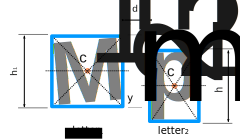
\includegraphics[trim= 200px 280px 300px 220px, clip, width=0.75\textwidth]{letter_position.pdf}
		\caption[Text letter horizontal and vertical alignments]{Letter horizontal and vertical positions variables (on the left $letter_1$, on the right $letter_2$). The two rectangles represent the bounding boxes and $c1$ and $c2$ their centres.}
		\label{fig:se:letter_position}
	\end{figure}
	%%%%%%%%%%%%%%%%%%%%%%%%%%%%%%%%%%%%%%%%%%%%%%%%%%%


 This is similar in principle to~\cite{Clavelli09} but adapted to take into account the horizontal alignment of text lines. Our method does not consider the letter width as we never know how many letters correspond to the CC.
 It can easily be used for vertical text by switching horizontal and vertical measurements.



	% paragraph pruning (end)


\paragraph{Text line construction} % (fold)
\label{par:se:letter_to_line}

TODO (already published somewhere...) 

% paragraph classification (end)

% section panel_and_text (end)

\section{From text to balloon} % (fold)
\label{sec:se:from_text_to_balloon}
% In this section we detail a novel approach for closed and non-closed speech balloon localization in scanned comic book pages, an essential step towards a fully automatic comic book understanding. 
For comics content understanding, speech balloons present a lot of interest since they offer the links between the textual content and the comic characters providing information about the localization of the characters and the tone of speech. 
As mentioned in section~\ref{??}, speech balloons are the more frequent type of balloon in comics and are highly related to speech text regions.
In this section we propose two approaches for balloon extraction based on text region location that can be detected using the methods presented in section~\ref{sec:se:panel_and_text} or~\ref{sec:in:text_localisation_and_recognition}.
The first method defined as ``balloon'' the smallest connected-components contains several text regions.
The second method groups text lines into paragraphs and initializes an active contour model (snake) on its outline.
From the initial position, the snake is pushed away from the text and attracted by surrounding edges at the same time in order to stick to any potential balloon stroke close by.
The main advantage of the second method is its ability to detect implicit or partially drawn balloons as well as the closed ones.

\subsection{Regular balloon extraction} % (fold)
\label{sub:se:regular_balloon_extraction}
Regular balloon are defined as closed balloon with a completely drawn contour unlike implicit contour discussed in the next subsection~\ref{sub:se:implicit_balloon_extraction}.
Closed balloon are easily extractable using blob detection method similarly to the panel and text extraction presented above.
The main different lies in their dominant colour with is white and implies do extract white connected-components instead of black for panels and text.
One particularity of text inside balloons is its vertical and/or horizontal alignment in the balloon (Figure~\ref{fig:se:text_in_balloon}).
We propose to use this characteristic to compute a confidence value to each connected-component that include one or more text regions.

	%%%%%%%%%%%%%%%%%%%%%%%%%%%%%%%%%%%%%%%%%%%%%%%%%%%
	\begin{figure}[h!]	%trim=l b r t  width=0.5\textwidth,
	  \centering
		\includegraphics[trim= 0px 0px 0px 0px, clip, width=0.75\textwidth]{text_in_balloon.png}
		\caption[Text positions in speech balloons]{Example of text positions in speech balloons.}
		\label{fig:se:text_in_balloon}
	\end{figure}
	%%%%%%%%%%%%%%%%%%%%%%%%%%%%%%%%%%%%%%%%%%%%%%%%%%%

% The alignment confidence can be used in a later stage to classify balloon and non regions.
\paragraph{Blob extraction} % (fold)
\label{par:blob_extraction}

A typical ``closed'' balloon is surrounded by a black stroke that defined a white region (blob) inside it, with holes created by the presence of text letters.
We propose to make a binary segmentation of the comics image and then use connected-component labelling method to extract white blobs (Figure~\ref{fig:se:closed_balloon}).
Closed balloons are usually surrounded by a black stroke with no difference from one to another in a given image.
We use a global binary segmentation method to separate the page background from its content (black strokes).
Here, we do not use a local segmentation approach because it has more chances to split the balloon border and over-segment them.

	%%%%%%%%%%%%%%%%%%%%%%%%%%%%%%%%%%%%%%%%%%%%%%%%%%%
	\begin{figure}[h!]	%trim=l b r t  width=0.5\textwidth,
	  \centering
		\includegraphics[trim= 0px 0px 0px 0px, clip, width=0.75\textwidth]{closed_balloon_process.png}
		\caption[Sequential balloon extraction process illustration]{Balloon extraction process. Original image, binary segmentation, contour detection (connected components) and result mask from left to right.}
		\label{fig:se:closed_balloon}
	\end{figure}
	%%%%%%%%%%%%%%%%%%%%%%%%%%%%%%%%%%%%%%%%%%%%%%%%%%%


% paragraph blob_extraction (end)

\paragraph{Text line grouping} % (fold)
\label{par:text_line_grouping}

As we are interested in localizing balloons from text, we post-process the results of the text line detection to group text lines into text area (paragraph), according to two rules.
First, we require that the candidate text lines to group have similar heights (or width in case of vertical text) and second that the inter-line distance is smaller than the average text line height of the potential paragraph region (Figure~\ref{fig:se:line_to_paragraphs}).

	%%%%%%%%%%%%%%%%%%%%%%%%%%%%%%%%%%%%%%%%%%%%%%%%%%%
	\begin{figure}[h!]	%trim=l b r t  width=0.5\textwidth,
	  \centering
		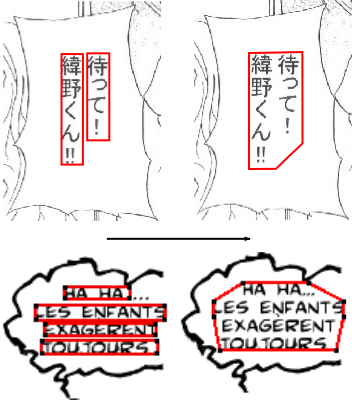
\includegraphics[trim= 0px 0px 0px 0px, clip, width=0.5\textwidth]{line_to_paragraphs.pdf}
		\caption[Text line to text paragraph conversion illustration]{Illustration of the text line to text paragraph conversion from left to right for vertical and horizontal text.}
		\label{fig:se:line_to_paragraphs}
	\end{figure}
	%%%%%%%%%%%%%%%%%%%%%%%%%%%%%%%%%%%%%%%%%%%%%%%%%%%

% paragraph text_line_grouping (end)

\paragraph{Balloon extraction} % (fold)
\label{par:balloon_extraction}

For each extracted blob that includes a text paragraph (one or more text lines), we compute the difference of alignment $C_{balloon}$ on the horizontal $d_x$ and the vertical $d_y$ axis between the balloon barycentre $c_1$ and the text paragraph barycentre $c_2$ (Figure~\ref{fig:se:align_diff}).

	%%%%%%%%%%%%%%%%%%%%%%%%%%%%%%%%%%%%%%%%%%%%%%%%%%%
	\begin{figure}[h!]	%trim=l b r t  width=0.5\textwidth,
	  \centering
		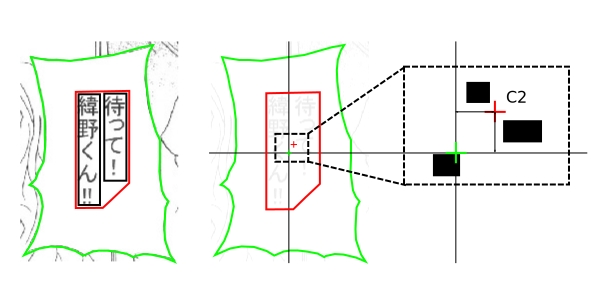
\includegraphics[trim= 140px 0px 0px 0px, clip, width=0.5\textwidth]{text_balloon_alignment.pdf}
		\caption[Illustration of the vertical and horizontal alignment differences between balloon and text region barycentre]{Vertical $d_y$ and horizontal $d_x$ alignment differences between balloon barycentre $c_1$ and text region barycentre $c_2$.}
		\label{fig:se:align_diff}
	\end{figure}
	%%%%%%%%%%%%%%%%%%%%%%%%%%%%%%%%%%%%%%%%%%%%%%%%%%%

Both differences $dx$ and $dy$ are normalized between zero and one as a percentage of the balloon width $B_{width}$ and height $B_{height}$ respectively.
The average of the vertical and horizontal alignments gives a confidence value for each balloon candidate, see formula~\ref{eq:se:balloon_confidence_value}.


\begin{equation}
	\label{eq:se:balloon_confidence_value}
	C_{balloon} = 1 - \frac{1}{2} *  \bigg( \frac{d_x}{B_{width}} + \frac{d_y}{B_{height}} \bigg)
\end{equation}

Balloon confidence value is used for balloon and non balloon classification in~\ch{chap:experimentations}.

% paragraph balloon_extraction (end)


% subsection regular_balloon_extraction (end)

\subsection{Implicit balloon extraction} % (fold)
\label{sub:se:implicit_balloon_extraction}

Balloon contour is not always completely drawn, it may be implied by contrast difference or other surrounding elements (Figure~\ref{fig:se:balloon_examples}c).
In most of the cases, including when contours are implicit, the location of text is generally a good clue to guess where the balloon is.
The problem of speech balloon outline detection can therefore be posed as the fitting of a closed contour around text areas, with the distinctiveness that the outline might not be explicitly defined in the image.
For the examples given in Figure~\ref{fig:se:balloon_examples}, this would be a smooth contour with relatively constant curvature (Figure~\ref{fig:se:balloon_examples}a), an irregular one with high local curvature (Figure~\ref{fig:se:balloon_examples}b), and an implicit one with missing parts (Figure~\ref{fig:se:balloon_examples}c).

	%%%%%%%%%%%%%%%%%%%%%%%%%%%%%%%%%%%%%%%%%%%%%%%%%%%
	\begin{figure}[!ht]%trim=l b r t  width=0.5\textwidth,
	\begin{center}
	  \begin{tabular}{ccc}
	  \includegraphics[trim= 0px 2px 0mm 0mm, clip, width=0.13\textwidth]{round_balloon.png}&
	  \includegraphics[trim= 0mm 0mm 0mm 0mm, clip, width=0.17\textwidth]{peaked_balloon.png}&
	  \includegraphics[trim= 15px 7mm 5px 0mm, clip, width=0.145\textwidth]{open_balloon.png} \\ 
	  \footnotesize a) Smooth	& \footnotesize b) Irregular & \footnotesize c) Implicit
	  \end{tabular}
	\caption[Speech balloon contour types]{Example of speech balloons with different contour types. Image credits~\cite{Bubble09}.}
	\label{fig:se:balloon_examples}
	\end{center}
	\end{figure}	
	%%%%%%%%%%%%%%%%%%%%%%%%%%%%%%%%%%%%%%%%%%%%%%%%%%%

Observing the heterogeneity of balloons, and considering the difficulty to manage ``open'' or ``implicit'' balloons, it appears necessary to use a dynamic and adaptive outline detection algorithm.
Active contours appear to be suitable to the problem.
The active contour framework was developed for delineating an object outline in an image.
The algorithm attempts to minimize the energy associated to the current contour, defined as the sum of an internal and an external energy term. 
In this paper we propose two adaptations of the active contour theory to the domain of comic balloon detection.
Specifically, we handle the case of balloons with missing parts or implicit contours, while we adopt a two-step approach to fit irregular outline types such as peak and cloud type balloons. 
To achieve this, we propose new energy terms making use of domain knowledge.


%------------------------------------------------------------------------
\subsubsection{Active contours}
\label{sec:se:active_contour}

The active contour~\cite{Kass1988} model is a deformable model, also known as snake, corresponding to a curve $\mathbf{v}(s)=[x(s),y(s)], s \in [0,1]$, that moves through the spatial domain of an image to minimize the energy functional (equation~\ref{eq:se:energy1}).

\begin{equation}\label{eq:se:energy1}
  E = \int_0^1 \! \frac{1}{2} \left( \alpha \left|\mathbf{v}'(s) \right|^2 + \beta \left| \mathbf{v}''(s) \right|^2 \right) + E_{ext}(\mathbf{v}(s))ds\\
\end{equation}
where $\alpha$ and $\beta$ are weighting parameters that respectively control the snake's tension and rigidity, and $\mathbf{v}'$ and $\mathbf{v}''$ denote the first and second derivatives of $\mathbf{v}(s)$ with respect to $s$. This functional energy is also called $E_{int}$ for internal energy.
The external energy function $E_{ext}$ is computed from the image so that it takes on its smaller values at the features of interest, such as boundaries~\cite{Xu1998}.
%It was initially designed to localize nearby edges accurately by using both internal and external energies (see eq.~\ref{eq:se:energy1}). 
%The external energy function $E_{ext}$ aim to attract the snake to the feature of interest (e.g. line, edge, corner), it is the image force. 
One of the proposed energy functions by Kass~\cite{Kass1988} is equation~\ref{eq:se:edge} which attracts the contour to edges with large image gradients. 
\begin{equation}\label{eq:se:edge}
  E_{ext} = -|\nabla \mathbf{I}(x,y)^2|
\end{equation}

We adapt the active contour framework to the domain of comics to detect speech balloons given a prior detection of text regions, introducing new energy terms based on domain knowledge about the relationship between text and balloons.
For the discussion below, we assume that text has been already detected in the image, see section~\ref{sec:se:panel_and_text} or~\ref{sec:in:text}.% and we use the method of \cite{Rigaud2013VISAPP} for text detection.

The introduction of statistical shape knowledge has already been studied in the literature~\cite{Cremers2002} but can not be applied here because of the lack of knowledge about the contour shape to detect.
Hence we introduce a new energy term, denoted $E_{text}$ (see equation~\ref{eq:se:energy2}) that conveys information about the relative placement of the balloon outline and the enclosed text.

\begin{equation}\label{eq:se:energy2}
  E = E_{int} + E_{ext} + E_{text}\\
\end{equation}

\subsubsection{External energy}
\label{sec:se:external_energie}
%The external energy $E_{ext}$ encourage curve onto image structures (e.g. edges, line, corner).

We consider edges as features of interest because we expect the speech balloon to be delimited by strong edges, at least partially.
Here we perform edge detection using the well know Sobel operator (Figure~\ref{fig:se:distance_transform}).
The original Kass~\cite{Kass1988} external energy (Equation~\ref{eq:se:edge}) is appropriate for natural scene images with smooth gradients but not for stroke-based images such as comics that comprise uniform coloured regions with strong edges.
In our case, we require that edges attract the snake from relatively far away (distances where the original edge gradient has already dropped to zero).
The method of Xu~\cite{Xu1998} would be appropriate here, although we have decided to use the equivalent distance transform of the edge image instead for computational efficiency reasons.
We therefore define the external energy function as:

\begin{equation}\label{eq:se:energy3}
  E_{ext} = \gamma \min A(i,j) = \gamma \min  \sqrt{(x_i-x_j)^2+(y_i-y_j)^2}\\
\end{equation}
where $E_{ext}$ is the minimum Euclidean distance ($A$) between a point $i$ and the nearest edge point $j$, $\gamma$ is a weighting parameter.

Since it is not desirable for edges corresponding to text to attract the snake, any edges that fall within the text regions are removed before the distance transform is calculated and do not contribute to the external energy.
	
	%%%%%%%%%%%%%%%%%%%%%%%%%%%%%%%%%%%%%%%%%%%%%%%%%%%
	\begin{figure}[!ht]	%trim=l b r t  width=0.5\textwidth,
	  \centering
		\fbox{\includegraphics[trim = 0mm 0mm 7mm 0mm, clip, width=230px]{edge_dist_trans.png}}
		\caption[Active contour energies for open balloon extraction]{Example of original image (top left) and its corresponding non-text edge detection (top right), $E_{ext}$ energy (bottom-left) and $E_{text}$ energy (bottom-right). In the bottom part, white corresponds to high energy.}
		\label{fig:se:distance_transform}
	\end{figure}
	%%%%%%%%%%%%%%%%%%%%%%%%%%%%%%%%%%%%%%%%%%%%%%%%%%%

\subsubsection{Internal energy}
We use the original definition of the internal energy (see equation~\ref{eq:se:energy1}) which can by decomposed in two energy terms: $E_{cont} = \left|\mathbf{v}'(s) \right|^2$ and $E_{curv}=\left| \mathbf{v}''(s) \right|^2$.
%It is composed of a continuity and a curvature energies: $E_{internal} = \alpha E_{cont} + \beta E_{curv}$ as defined in eq.~\ref{eq:se:energy3}. The coefficients $\alpha$ and $\beta$ give more or less importance to one energy or another.
% 
% \begin{equation}\label{eq:se:energy3}
%   E_{internal} = \left( \alpha(s)  \left|\frac{d\bar{v}}{ds}(s) \right|^2 + \beta(s) \left| \frac{d^2\bar{v}}{ds^2}(s) \right|^2 \right) /2
% \end{equation}

The energy $E_{cont}$ forces the contour to be continuous by keeping points at equal distance, spreading them equally along the snake according to the average inter-point distance of the contour.
It becomes small when the distance between consecutive points is close to the average, see equation~\ref{eq:se:cont}.

\begin{equation}\label{eq:se:cont}
 E_{cont} = \alpha \Big|\bar{d} - \sqrt{(x_i - x_{i-1} )^2 + (y_i - y_{i-1} )^2}\Big|
\end{equation}
where $\bar{d}$ is the average distance between two consecutive points $i$ and $j$ of the snake and $\alpha$ is a weighting parameter.

The energy $E_{curv}$ enforces smoothness and avoids oscillations of the snake by penalizing high contour curvatures (minimizing the second derivative).
It becomes small when the angle between three points is close to zero, see equation~\ref{eq:se:curv}.
% Note, this energy itself makes the snake deflate and converge to a line or a point.

\begin{equation}\label{eq:se:curv}
  %E_{curv} = \beta | p_{i-1} - 2 * p_i + p_{i+1} |^2
  E_{curv} = \beta \left( (x_{i-1} - 2x_{i} + x_{i+1})^2 + (y_{i-1} - 2y_{i} + y_{i+1})^2 \right)
\end{equation}
where $i$ is a point of the snake and $\beta$ a weighting parameter.

%The distance $h1$ is an a priori distance between the text and its balloon. % for positioning the snake when there is a lake of external energy at low resolution detection.
%The distance $h2$ is the difference between the outer and the inner distance

\subsubsection{Text energy}
\label{sec:se:text_energie}

The text energy $E_{text}$ conveys domain specific knowledge about the relative locations of text areas and their associated balloon contours.
It is necessary in this domain to consider the lack of explicit information in the cases of implicit balloons, where parts of the outline are missing.
The $E_{text}$ energy aims at pushing the snake outwards toward the most likely balloon localization, given the position of the text area.
This energy term has two effects.
First, it acts collaboratively to the external energy, by moving the snake towards non-text edges (hopefully corresponding to the balloon outline).
Second, in the case of implied contours where no explicit edge exists (the external energy term is not informative), $E_{text}$ assists the algorithm to converge to an approximate contour position based on prior knowledge on the expected localization given the corresponding text area.
We define the text energy term at a localization $i$ of the image as follows:

\begin{equation}\label{eq:se:know}
E_{text} = \begin{cases} \kappa \frac{N}{min_{j \in T} A(i,j)} & \mbox{if } A(i,j) > 0 \\ \kappa N & \mbox{else} \end{cases}
\end{equation}
where $j$ is a pixel in the text area $T$, $N$ is an experimentally defined constant expressing the expected distance in pixel between the text area and the corresponding balloon boundary and $\kappa$ is a weighting parameter that controls the contribution of $E_{text}$ with respect to the other energy terms in eq.~\ref{eq:se:energy2}. Note when $i$ is on the border of $T$, the distance $A(i,j)$ is equal zero and the energy becomes maximal as if it was inside $T$.


\subsubsection{Proposed method}
\label{sec:proposed_method}

In this section we detail how to localize speech balloons using active contours based on the definitions given above. 
First we generate the static external energy map $E_{ext}$ for the whole image and then for each text area we compute the $E_{text}$ energy.
The internal energy $E_{int}$ is calculated for each point of the snake before each iteration.
We iteratively examine each point of the snake in a clockwise fashion and move it within a neighbourhood region of size $M$ in order to minimize equation~\ref{eq:se:energy2}.
This operation is repeated until no point moves in one turn (see algorithm~\ref{al:be:method}).
We perform a first smooth-contour approximation of the balloon boundary (low resolution) and then we fit the contour better to the balloon shape (high resolution) using the same algorithm

TODO: remove high resolution step???
%, especially for non-smooth boundaries.% High resolution contour shape fitting - aiming to 
 %\item Contour classification [NOVELTY? SHAPE COMPOSED BY DIFFERENT PART OF SHAPE]

\begin{algorithm}
\caption{Open balloon detection loop}
\label{al:be:method}
\begin{algorithmic}
%\REQUIRE $n \geq 0 \vee x \neq 0$
%\ENSURE $y = x^n$
%\STATE $y \leftarrow 1$
\STATE{compute $E_{ext}$ energy}
\FOR{each text area}
  \STATE compute $E_{text}$ energy
  \STATE active contour initialization
  \STATE stop = False
  \WHILE{stop = False}%\STATE{DO}
    \STATE $n = 0$
    \FOR{each points of the snake}
      \STATE examine neighbourhood position energies
      \IF{one position reduce the current energy}
		\STATE move point to this position
		\STATE $n=n+1$
      \ENDIF
    \ENDFOR
    % \STATE // If not points have been moved then stop
    \IF{$n = 0$}
    	\STATE{stop = True}
    \ENDIF
  \ENDWHILE% <--- use \doWhile for the "while" at the end %\While{$n > 0$}
\ENDFOR
\end{algorithmic}
\end{algorithm}

\subsubsection{Active contour initialisation}
\label{sec:se:cont_init}

The active contour is initialized on the outline of the text paragraph region.
This corresponds to the convex hull of all the text lines that are included in the balloon (Figure~\ref{fig:se:paragraphs}b).
Note that the convex hull of the text area also corresponds to the $E_{text}$ maximal value border (Figure~\ref{fig:se:distance_transform}).
%At this point, the $E_{text}$ has to be the strongest in eq.~\ref{eq:se:energy2} in order to ``push'' away the snake from the text area and then facilitate its attraction by $E_{ext}$ (non text edges).
%Another possible initialization strategy could be to use the smaller ellipse circumscribing the text area.% This has been experimented section~\ref{sec:experiments}.

%Note, in case of wrong initialization, the external energy allow the snake to inflate deflate in the case of the snake initialization is outside the balloon. Gradients that are inside the initial curve repulsed the contour (considered as text areas).


%\subsubsection{Number of points}
The initial number of points impacts the way that the snake moves and the precision of the final detection.
During the first low resolution localization step, we perform a spaced equipartition of the points (Figure~\ref{fig:se:paragraphs}c) to quickly localize the global shape avoiding unnecessary stops on image details.
In the subsequent high resolution fitting stage, we add more intermediate points to fit the exact shape more precisely.
% with an inter-points distance fixed to half line height

%%%%%%%%%%%%%%%%%%%%%%%%%%%%%%%%%%%%%%%%%%%%%%%%%%%
	\begin{figure}[!ht]%trim=l b r t  width=0.5\textwidth,
	\begin{center}
	  \begin{tabular}{ccc}
	  \includegraphics[trim= 0mm 0mm 0mm 0mm, clip, width=0.20\textwidth]{group_lines.png}&
	  \includegraphics[trim= 0mm 0mm 0mm 0mm, clip, width=0.20\textwidth]{convex_hull.png}&
	  \includegraphics[trim= 48mm 0mm 0mm 0mm, clip, width=0.20\textwidth]{snake_init.png} \\ 
	  \footnotesize a) Group of text lines	& \footnotesize b) Text area convex hull 	& \footnotesize c) Snake initialization 
	  \end{tabular}
	\caption[Active contour initialization based on text region convex hull]{Active contour initialization based on text region convex hull.}
		\label{fig:se:paragraphs}
	\end{center}
	\end{figure}	
	%%%%%%%%%%%%%%%%%%%%%%%%%%%%%%%%%%%%%%%%%%%%%%%%%%%


%We initialize the active contour of $N$ points on the paragraph shape (group of lines) figure~\ref{fig:se:paragraphs} and then we make it grow until it hits edges.
%We define a paragraph as a group of text lines spoken by the same speaker and with no interruptions (e.g. time break, interaction, other person talk). These group of lines are written close to each other by convention . We labelize two consecutive lines as part of the same paragraph if there is no enough space for an other line similar in height between them.

\subsubsection{Low resolution contour localization}
Following a two stage process, we first aim to obtain a rough localization of the balloons by fitting a smooth contour using a few contour points during initialization.
The idea is to progressively push the snake away from the text area and towards the balloon boundary giving an increased weight to both the $E_{ext}$ and $E_{text}$ energy terms.
If the balloon has an explicit boundary then $E_{ext}$ will attract the snake to it.
If there is no explicit contour close enough to attract the snake then the $E_{text}$ term will push the snake to the suggested position of the balloon contour.
Also the internal energies are important at this stage to maintain a certain rigidity of the snake.
%The and low external energy parameter $\gamma$, a large internal curvature energy parameter $\beta$ and a large knowledge energy parameter $\eta$ (Fig.~\ref{fig:se:multiscale01}). 
At the end of this step, we obtain a preliminary localization of the speech balloons (Figure~\ref{fig:se:mono_res_det}). 

	%%%%%%%%%%%%%%%%%%%%%%%%%%%%%%%%%%%%%%%%%%%%%%%%%%%
	\begin{figure}[!ht]	%trim=l b r t  width=0.5\textwidth,
	  \centering
		% \fbox{
		\includegraphics[trim = 0mm 3mm 0mm 1mm, clip, width=220px]{mono_res_det.png}
		% }
		\caption[Examples of low resolution contour detection for balloon extraction]{Example of low resolution contour detection (red line) for irregular closed (left) and smooth open (right) balloons.}
		\label{fig:se:mono_res_det}
	\end{figure}
	%%%%%%%%%%%%%%%%%%%%%%%%%%%%%%%%%%%%%%%%%%%%%%%%%%%

% \subsection{Candidate point selection}
% {\bf SECTION REMOVED because we don't know yet how to efficiently select the point and because multi-resolution method already improves results without using candidate point selection. We can mention it in the prospects.}

%The candidate point selection aim to determine if the snake segments between points can be more detailed or not (e.g. detection of peak, circle, tail). Figure~\ref{fig:se:multiscale01} shown two categories of points, those who has been attracted and stopped by edge (part of the real contour) and the others (part of the suggested contour). At this point we can see that adding more points on the real contour parts and relaxing the internal energies could improve the contour detection. This a true but then all the contour will be affected and we could degrade the suggested contour detection part if it is a non closed contour. Therefore we add new points only between those stopped by edge because we can not get more detail about suggested parts of the contour and we could even loose the low resolution detection information.
%We consider as ``stopped'' the points that are common with the ``text less'' edge map (left part of fig.~\ref{fig:se:distance_transform}).
 %An example of candidate points is on figure~\ref{fig:se:multiscale01} and~\ref{fig:se:multiscale02}). We keep those new generated points only if they hit and edge before the snake stabilize again (only if they improve the contour detection). The aim is to get a higher resolution contour detection only where there is a contour drawn. If no contour (non closed balloon case) then we keep the appropriate shape from low resolution detection.


\subsubsection{High resolution contour shape fitting}
Figure~\ref{fig:se:mono_res_det} shows that the global shape of the top balloon has been detected although it is still far from a perfect fit because, as we can see on bottom part of the balloon, the snake was not able to fit precisely balloon outline, for instance peaky and tail regions are not well segmented.
To achieve a better fitting, we increase the resolution of the snake by adding new points between the current ones and by changing the weighting parameters of the energy function, and go through a second fitting process.
At this stage, we relax the $E_{curv}$ energy to make the snake to thinner parts of the boundary and we set $E_{cont}$ strong enough to keep a regular inter-point distance all over the contour.
Also, we reduce the $E_{text}$ energy weight because at this step, the snake is already far from text and this term is not informative any more.
%to give more importance to the image energy than the prior knowledge. %is reduced because  external  avoid point  is closer to the final contour and do not need the $E_{know}$ energy start to minimize we reduced the inter-points distance, we also increase the external energy parameter $\gamma$ to make the snake more attractable by image edge, decrease the internal curvature energy parameter $\beta$ to allow more flexible contour fitting and decrease the knowledge energy parameter $\eta$ because the contour is now far from the text. 
This new configuration allows the snake to fit more precisely to the balloon contour as shown in figure~\ref{fig:se:hd_contour} (to compare with figure~\ref{fig:se:mono_res_det}).

%{\bf TO ADD IF RESULTS CONFIRMS: we consider external energy map based from edge detection only (no distance transform any more)?}

	%%%%%%%%%%%%%%%%%%%%%%%%%%%%%%%%%%%%%%%%%%%%%%%%%%%
	\begin{figure}[!ht]	%trim=l b r t  width=0.5\textwidth,
	  \centering
		\fbox{\includegraphics[trim = 0mm 2mm 0mm 1mm, clip, width=180px]{multi_res_det.png}}
		\caption[Examples of high resolution contour detection for balloon extraction]{Examples of high resolution contour detection (red line) for closed (left) and open (right) balloons.}
		\label{fig:se:hd_contour}
	\end{figure}
	%%%%%%%%%%%%%%%%%%%%%%%%%%%%%%%%%%%%%%%%%%%%%%%%%%%

% subsection implicit_balloon_extraction (end)

% section from_text_to_balloon_ (end)

\section{From balloon to tail} % (fold)
\label{sec:se:from_balloon_to_tail}

Speech balloons indicate dialogue with tails pointing at their respective speakers~\cite{Varnum2007Language}
%Balloon tails tell the reader the relationships between a set of textual or graphic elements contained in the speech balloons and the comics characters [REF???].
, usually represented by a discontinuity on balloon contour (Figure~\ref{fig:se:tail_types}). 
We propose to detect the tail position and direction based on the balloon contour analysis.
We limit this study to the tail types that can be considered has an extension of the inside region (background) of the speech balloon namely types ``comma'', ``zigzag'' and ``absent'' in Figure~\ref{fig:se:tail_types} because they can all be extracted from the segmentation of the balloon background.
Other types require a specific study from the speech balloon extraction that should consider the contour stroke and surrounding elements.

    %%%%%%%%%%%%%%%%%%%%%%%%%%%%%%%%%%%%%%%%%%%%%%%%%%%%%%%%
    \begin{figure}[ht]%trim=l b r t  width=0.5\textwidth,  
      \centering
      \includegraphics[trim= 0px 0px 0mm 0mm, clip, width=0.75\textwidth]{tail_types.png}
    \caption[Examples of type of speech balloon tails]{Examples of type of speech balloon tails. From left to right: stroke, comma, circle, zigzag, absent.}
    \label{fig:se:tail_types}
    \end{figure}
    %%%%%%%%%%%%%%%%%%%%%%%%%%%%%%%%%%%%%%%%%%%%%%%%%%%%%%%%

We propose a method to describe ``comma'', ``zigzag'' and ``absent'' (no tail) types.
The tail can be decomposed into four elements: origin, path, tip and pointed direction.
The contour of a speech balloon is mainly convex except in the region where the tail is connected to the balloon (origin) which produces the highest convexity defects.
If the speech balloon has no tail, there is no particular convexity defect.
% and we can also detect it, see the end of this subsection.
%We propose to detect the two biggest convexity defects to locate the tail origin.
A convexity defect is defined by a triangle from one segment of the balloon convex hull to the farthest point on the balloon contour (Figure~\ref{fig:se:convexity_defects}).
The set $F=\{f_0,f_1,...f_n\}$ represents farthest points from the corresponding hull segments $S=\{s_0, s_1,...,s_n\}$ where $n$ is the number of hull segments.
We define the top two farthest points $f_a$ and $f_b$ corresponding to the convex hull segments $s_a$ and $s_b$, as the coordinates of the tail origin (Figure~\ref{fig:se:convexity_defects}).

    %%%%%%%%%%%%%%%%%%%%%%%%%%%%%%%%%%%%%%%%%%%%%%%%%%%%%%%%
    \begin{figure}[ht]%trim=l b r t  width=0.5\textwidth,  
      \centering
      
\includegraphics[width=0.9\textwidth]{tail_description.pdf}
    \caption[Representation of the two biggest convexity defects that defines the tail origin]{Representation of the two biggest convexity defects that defines the tail origin $f_a$ and $f_b$ (left). On the right side, we represent the distances related to the vertex $v_7$ to illustrate the variables of equation~\ref{eq:se:optimisation}. In this case $ds_b=0$ because $v_7$ coincides with an end of segment $s_b$ (distance equal to zero).}
    \label{fig:se:convexity_defects}
    \end{figure}
    %%%%%%%%%%%%%%%%%%%%%%%%%%%%%%%%%%%%%%%%%%%%%%%%%%%%%%%%

Most of the time, the tail tip corresponds to one of the vertices of the convex hull.
We define the set of vertices $V=\{v_1,v_2,...,$ $v_n\}$.
The optimal vertex is computed by comparing five features that corresponds to the Euclidean distances:

\begin{itemize}
   \item $ds_a$ the distance to the segment $s_a$
   \item $ds_b$ the distance to the segment $s_b$
   \item $dc$ the distance to the centre of mass $c$ of the balloon
   \item $df_a$ the distance to the tail origin $f_a$
   \item $df_b$ the distance to the tail origin $f_b$
 \end{itemize} 

This can be formulated as:
\begin{equation}\label{eq:se:optimisation}
   v* = argmax\big( max(dc+df_a+df_b) + min(ds_a + ds_b) \big)\\
 \end{equation}
 where $v*$ is the optimal vertex from the set of vertex $V$.
%NEW IDEA: for all the vertex between the two defects, min/max a feature vector (dist to barycentre, distance to tail origin).
% Most of the time both triangles intersect on the same point which is the tail tip $T$.
% If not, we determine which pair of points from the two segments that are the closest ($t_1$ and $t_2$) and then which one is the tail tip ($t_1$ or $t_2$).
% The tail tip is defined by the farthest from the tail origin:
% $T = \begin{cases} t_1, & \mbox{if } dist(f_1,t_1) > dist(f_2,t_2) \\ t_2, & \mbox{else} \end{cases}$
%Each segment of the convect hull has a convexity defect that we $cd_i$ 

Together with the position, we compute a confidence value $C_{tail}$ related to the mean depth of $f_a$ and $f_b$ over the mean balloon size $meanBalloonSize$, see formula~\ref{eq:se:confidence_tail}.

\begin{equation}
\label{eq:se:confidence_tail}
  C_{tail} = \frac{(depth(f_a)+depth(f_b))/2}{meanBalloonSize}
\end{equation}
where $depth(f_x)$ is the depth of the corresponding defect in number of pixels and $meanBalloonSize$ is defined in equation~\ref{eq:se:mean_balloon_size}.


\begin{equation}
  \label{eq:se:mean_balloon_size}
  meanBalloonSize = \frac{\sum\limits_{i=0}^n Wb_i + \sum\limits_{i=0}^n Hb_i}{n * 2}  
\end{equation}
where $Wb_i$ and $Hb_i$ correspond to the width and the height of a speech  balloon $i$ and $n$ the number of speech balloons in the image.

% By measuring the variance in of all the convexity defect distances $\sum\limits_{i=0}^n var(f_i)$ of the contour we can detect if there is a tail or not, see equation~\ref{eq:se:var_defects}.
% We use a fixed threshold of $thV=10\%$ of the balloon height to decide if a balloon has a tail or not, see equation~\ref{eq:se:var_defects}.

% \begin{equation}
% \label{eq:se:var_defects}
%   hasTail = \begin{cases} 1, & \mbox{ if } \sum\limits_{i=0}^n var(f_i) > thV \\ 0, & \mbox{ else}  \end{cases}
% \end{equation}
% where $thV$ is a decision threshold relative to the average balloon size in the image.

Once we find the tail tip, we analyse its neighbourhood to find the orientation and the direction of the last part of the tail which is directed towards the speaking character.
We compute a $M$x$M$ square region centred on the tail tip position in the balloon mask and use a line fitting algorithm (weighted least-squares) that returns the representative line that minimizes the distance between all the points of the local region (Figure~\ref{fig:se:orientation}).


    %%%%%%%%%%%%%%%%%%%%%%%%%%%%%%%%%%%%%%%%%%%%%%%%%%%%%%%%
    \begin{figure}[ht]%trim=l b r t  width=0.5\textwidth,  
      \centering
      \includegraphics[width=0.5\textwidth]{tail_direction.png}
    \caption[Tail orientation given by the line fitting algorithm in the neighbourhood of the tail tip]{Tail orientation given by the line fitting algorithm in the neighbourhood of the tail tip.}
    \label{fig:se:orientation}
    \end{figure}  
    %%%%%%%%%%%%%%%%%%%%%%%%%%%%%%%%%%%%%%%%%%%%%%%%%%%%%%%%


The tail direction is computed from the tail orientation that has initially two possible directions.
We define the tail direction from the closest point $fitLinePoint$ of the representative line to the tail origin, to the tail tip ($vec\{fitLinePoint,$ $tailTip\}$).
 %by selecting the vector that starts close to the $F$ points and ends far from the $F$ points:

%$\dot{\vec{p}} = m\vec{v}$
% $\vec{vec\{dir\}} = \begin{cases} vec\{x_1,x_2\}, & \mbox{if } d(f_1,x_1) + d(f_2,x_1) < d(f_1,x_2) + d(f_2,x_2) \\ vec\{x_2,x_1\}, & \mbox{else} \end{cases}$

% section from_balloon_to_tail (end)


%--------------------------------------------------------------------------------------------------------------------------------------
\section{From tail to comic character} % (fold)
\label{sec:se:tail_to_character}


%from_tail_to_comic_character detecting the characters, in their great diversity, from the drawings of a comic book's page is quite a piece of work, 
% To detect comic characters from the tail detection, we narrow down the panel region according to position of the tail tip and to direction it is pointed to.
% area where we are going to look for them in.
% This can be done thanks to the panel, balloon and tail detection we extracted on the image during the previous steps.
% We make the assumption that the main characters of a story speak at some point.
% We focus on the characters that are emitting a speech balloon (speaking characters) and try to localize them from the speech balloon informations.
% That is to say that speech balloons will be associated one or several times to each of the character in different panels.

As we know which balloons are in which panel (total inclusion), we can estimate from the position and direction of the tail, which part of the panel may contain the speaking character.
The tail orientation is quantized in eight cones of $\pi/4$ radius so we can consider that, in a rectangular-shaped panel (or its bounding box), the tail is either pointing towards a corner or towards a border of the panel.
We define the ROI for the character as a squared region beside the speech balloon.
The maximum width $w_{max}$ and height $h_{max}$ of the ROI are equal to the mean widths and heights of all the balloons in the image, see equation \ref{eq:se:mean_balloon_size}.

The position of the ROI around the speech balloon is defined by two opposite points of a square $A_{x,y}$ and $B_{x,y}$ according to formula~\ref{eq:se:roi_position_around_balloon} which is sometimes constrained by a panel border that is why the term $min()$ appears.
The different positions of the ROI are illustrated on figure \ref{fig:se:roi_area}.

\begin{equation}
  \label{eq:se:roi_position_around_balloon}
  \begin{array}{rccl} 
	  A_x & = & v^*_x - min(Pi_x - v^*_x, w_{max}) & * O_x \\ 
	  A_y & = & v^*_y - min(Pi_y - v^*_y, h_{max}) & * O_y \\ 
	  B_x & = & \left[ A_x + min(Pi_x - A_x, w_{max}) \right] & * O_x \\ 
	  B_y & = & \left[ A_y + min(Pi_y - A_y, h_{max}) \right] & * O_y
  \end{array} 
\end{equation}
where $v^*$ is the coordinates of the tail tip (see section~\ref{sec:tail_extraction}), $Pi$ the coordinates of one of the four corners of the panel bounding box $P=\{P0, P1, P2, P3\}$ and $O$ the offset for the direction of the tail.
The offset $O$ is quantized in heigh values according to the tail direction and the panel's corner $P_i$ is chosen accordingly, see table~\ref{tab:se:offset_panel_corner}.

    %%%%%%%%%%%%%%%%%%%%%%%%%%%%%%%%%%%%%%%%%%%%%%%%%%%
  \begin{table}[ht]
    \normalsize
%\renewcommand{\arraystretch}{1.2}

    \centering
    \caption{Values of the offset $O$ on horizontal and vertical axis and panel's corner selection according to the eight directions of the tail.}
    % \def\arraystretch{1.5}%  1 is the default, change whatever you need
    \setlength{\tabcolsep}{.45em}
    % \extracolsep{\fill}
    \begin{tabular}{|c|c|c|c|c|c|c|c|c|}

          \hline
	      &  N  & NE  & E  & SE & S & SW & W & NW   \\
	      \hline
	      $O_x$   & 0.5  & 0.75 & 1.0  & 0.75 & 0.5 & -0.75& -0.5 & 0.75  \\
	      \hline
	      $O_y$   & -1   & -0.75& -0.5 & 0.75 & 1.0 & 0.75 & -0.5 & -0.75  \\
	      \hline
	      $Pi$    & P1   & P1   & P1   & P1   & P3  & P3   & P3   & P3   \\
          \hline
        \end{tabular}
    \label{tab:se:offset_panel_corner}
  \end{table}%
    %%%%%%%%%%%%%%%%%%%%%%%%%%%%%%%%%%%%%%%%%%%%%%%%%%%


% Sometimes the pointed corner or border is far from the tail tip and create a wide region.

%An analysis of the eBDtheque ground truth gave us the confirmation that this estimated areas were actually containing more than 70\% of the characters with a precision of 50\% in average.

%%%%%%%%%%%%%%%%%%%%%%%%%%%%%%%%%%%%%%%%%%%%%%%%%%%
 \begin{figure}[!ht]
   \centering
  %\includegraphics[width=150px]{fig/roi_area.pdf}
  
\includegraphics[width=180px]{roi_hypothesis.pdf}
  \caption[Illustration of the character region of interested computation for each of the eight directions of the tail]{Illustration of a panel with four corners $P0, P1, P2, P3$ and the different ROI position and size that can be defined for each of the eight directions of the tail.
  }
  \label{fig:se:roi_area}
 \end{figure}
%%%%%%%%%%%%%%%%%%%%%%%%%%%%%%%%%%%%%%%%%%%%%%%%%%%

% The ROI are then passed to the comic character extractor (see section~\ref{sub:character_extraction}) which will locate more precisely the characters based on image features.
% image processing part (character extractor) that will spot all the characters, especially the ones that does not speak, using those regions as seeds.


% section from_tail_to_comic_character (end)

% Conclusion --------------------------------------------------------------------------------------------------------------------------------------
\section{Conclusions}
\label{sec:se:conclusion}
In this section we have presented how to understand comics image content by following the relations between elements, defined by knowledge domain.
This approach is quite natural, trying to reproduce the reader's reading behaviour: first to search for the panels and then speech balloons, read their content and make the link with the characters and other graphic in the panel.
Despite the intuitiveness of this approach, the main drawback of this sequential approach is the dependency of the processes which propagates errors.
The experiments section~\ref{sub:ex:sequential_information_extraction_evaluation} evaluates the processes that are proposed here.

% In this section we have presented and evaluated two methods for panel extraction based on connected-components labelling.
% The experiments shows that both approaches are really efficient for comics using gutter where there is no drawing between panels.
% The first method have been published for national and international audience~\cite{rigaud2012extraction,Rigaud2012LNCS} and the second method is part of an international journal publication [pending acceptance???].

% Then, the variance of each class is computed to check the homogeneity of the ROI. If the variance of the ``frame'' class is high, a specific algorithm~\cite{Khoi11} is applied in order to improve the previous steps (binarisation and/or classification). 

Next chapter is going to present a non sequential approach able to extract comics image content using independent processing in order to avoid error propagation.

% Also, an open balloon detection method based on speech text position will be presented.


% \begin{itemize}
% 	% \item Compute a confidence value between 0 and 1 for each panel: the inverse of overlapping percentage with other panels. (maximal when no overlap). This can replace the topological filtering by considering as correct the panel with a confidence > 0\%
% 	\item \url{/PhD/publication/2013/LNCS/robust_frame_and_text_extraction_from_comic_books/paper}
% 	\item IJDAR paper > panel extraction %\url{/PhD/Publications/CIFED_2012}
% \end{itemize}
